% document formatting
\documentclass[10pt]{article}
\usepackage[utf8]{inputenc}
\usepackage[left=1in,right=1in,top=1in,bottom=1in]{geometry}
\usepackage[T1]{fontenc}
\usepackage{xcolor}

% math symbols, etc.
\usepackage{amsmath, amsfonts, amssymb, amsthm}
\usepackage{dsfont}

% lists
\usepackage{enumerate, enumitem}
\usepackage{tabularx, multirow}

% images
\usepackage{graphicx} % for images
\usepackage{tikz}

% code blocks
% \usepackage{minted, listings} 

% verbatim greek
\usepackage{alphabeta}

\newcommand{\dd}{\text{d}}

\graphicspath{{./assets/images/Module 16}}

\title{02-680 Module 16 \\ \large{Essentials of Mathematics and Statistics}}
 
\author{Aidan Jan}

\date{\today}

\begin{document}
\maketitle

\section*{Graphical Representations of Random Variables}
\subsection*{Bayesian Networks}
Sometimes, we need a more complicated conditional description.  One way to do this is using a network (a graph).  Bayesian networks decompose \textbf{joint distributions} into a product of simpler conditional probabilities, capturing variable dependencies and enabling more efficient computation.
\begin{center}
    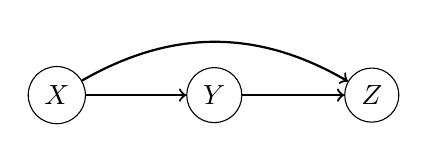
\begin{tikzpicture}
        \node[circle, draw] at (0, 0) (X) {$X$};
        \node[circle, draw] at (2, 0) (Y) {$Y$};
        \node[circle, draw] at (4, 0) (Z) {$Z$};

        \draw[->, thick] (X) -- (Y);
        \draw[->, thick] (Y) -- (Z);
        \draw[->, thick] (X) to[bend left] (Z);
    \end{tikzpicture}
\end{center}
Bayesian networks have some convenient properties:
\begin{itemize}
    \item They are a simple way to visualize the structure of a probabilistic model
    \item They can be used to design or motivate new kinds of statistical models.
    \item Inspection of the graph alone gives us insight into properties, e.g., conditional independence.
    \item Complex computations for inference and learning in statistical models can be expressed in terms of graphical manipulations.
\end{itemize}
Directed links (arrows) between two nodes (random variables) indicate conditional probabilities.  For example, the arrow between $X$ and $Y$ gives the conditional probability $p(Y|X)$.

\subsection*{Construction of Bayesian Networks}
Starting with an example, consider the joint distribution:
\[p(a, b, c) = p(c | a, b) p(b | a) p(a)\]
of three random variables $a$, $b$, $c$.  The factorization of the joint distribution tells us something about the relationship between the random variables:
\begin{itemize}
    \item $c$ depends directly on $a$ and $b$.
    \item $b$ depends directly on $a$.
    \item $a$ depends neither on $b$ nor on $c$.
\end{itemize}
Now, we can begin construction.  
\begin{enumerate}
    \item Create a node for all random variables
    \begin{center}
        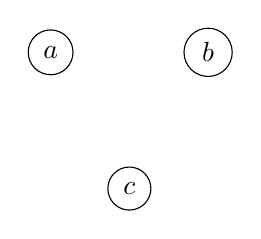
\begin{tikzpicture}
            \node[circle, draw] at (0, 0) (a) {$a$};
            \node[circle, draw] at (2, 0) (b) {$b$};
            \node[circle, draw] at (1, -1.73) (c) {$c$};
        \end{tikzpicture}
    \end{center}
    \item For each conditional distribution, we add a directed link (arrow) to the graph from the nodes corresponding to the variables on which the distribution is conditioned.
    \begin{center}
        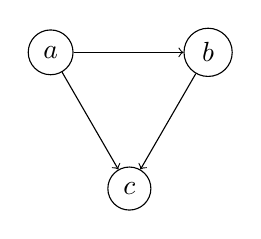
\begin{tikzpicture}
            \node[circle, draw] at (0, 0) (a) {$a$};
            \node[circle, draw] at (2, 0) (b) {$b$};
            \node[circle, draw] at (1, -1.73) (c) {$c$};
            \draw[->] (a) -- (b);
            \draw[->] (a) -- (c);
            \draw[->] (b) -- (c);
        \end{tikzpicture}
    \end{center}
\end{enumerate}
The graph layout depends on the choice of factorization of the joint distribution.\\\\
Now, for the reverse, consider the following network:
\begin{center}
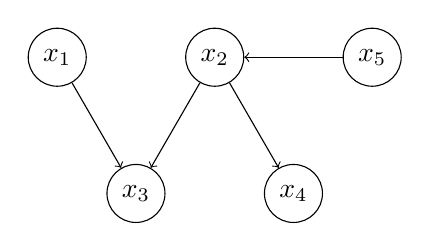
\begin{tikzpicture}
    \node[circle, draw] at (0, 0) (x1) {$x_1$};
    \node[circle, draw] at (2, 0) (x2) {$x_2$};
    \node[circle, draw] at (4, 0) (x5) {$x_5$};
    \node[circle, draw] at (1, -1.73) (x3) {$x_3$};
    \node[circle, draw] at (3, -1.73) (x4) {$x_4$};
    \draw[->] (x1) -- (x3);
    \draw[->] (x2) -- (x3);
    \draw[->] (x2) -- (x4);
    \draw[->] (x5) -- (x2);
\end{tikzpicture}
\end{center}
In this case, $x_1$ depends on nothing, $x_3$ depends on both $x_1$ and $x_2$, $x_2$ depends on $x_5$, $x_4$ depends on $x_2$, and $x_5$ depends on nothing.  We can therefore extract
\[p(x_1, x_2, x_3, x_4, x_5) = p(x_1) p(x_5) p(x_2 | x_5) p(x_3 | x_1, x_2) p(x_4 | x_2)\]

\subsection*{Joint Distributions}
In general, the joint distribution $p(x) = p(x_1, \dots, x_k)$ is given as
\[p(x) = \prod_{k = 1}^K p(x_k | \text{P}a_k)\]
where P$a_k$ means ``the \textbf{parent} nodes of $a_k$''.  \textbf{Parent} nodes of $a_k$ are nodes that have arrows pointing to $a_k$.\\\\
In general for a network, we define the probabilities as:
\[p\left(\langle Q_1, Q_2, \dots, Q_d \rangle\right) = \prod_{i = 0}^d p\left(Q_i \left| \bigwedge_{j \in N^{\text{in}}(Q_i)} Q_j\right.\right)\]
Note that $N^{\text{in}}(v)$ is the set of in-neighbors of $v$ in a graph.

\section*{Markov Chains}
A \textbf{Markov chain} is a special type of \textbf{stochastic process}, defined in terms of the conditional distributions of future states given the \textbf{present} and \textbf{past} states.\\\\
Markov chains are usually used to model sequences of items.  We saw when talking about conditional probabilities that:
\begin{align*}
    p(X_n, X_{n - 1}, \dots, X_1) &= p(X_n | X_{n - 1}, \dots, X_1)p(X_{n - 1}, \dots, X_1) \\
    &= p(X_n | X_{n - 1}, \dots, X_1) p(X_{n - 1} | X_{n - 2}, \dots, X_1) p(X_{n - 2}, \dots, X_1) \\
    &\dots \\
    &= p(X_n | X_{n - 1}, \dots, X_1) \dots p(X_2 | X_1) p(X_1)
\end{align*}
The \textbf{Markov assumption} is that the probability of $X_k$ depends on $X_{k - 1}$ alone.  This simplifies the computation, but at the cost of long term connections.  Anecdotally the Markov assumption says \textit{the future is independent of the past given the present.}\\\\
Therefore, we can rewrite the statement above as:
\[p(X_n, X_{n - 1}, \dots, X_1) = p(X_n | X_{n - 1}) p(X_{n - 1} | X_{n - 2}) \dots p(X_2 | X_1) p(X_1)\]
This is the basis for \textbf{Hidden Markov Models} which are used a lot in genetics.



\end{document}